\chapter{The Poisson problem}

\section{The Poisson problem}

The Poisson problem typically models a diffusion process, and is a very
important model problem in science and engineering. This is related to the fact
that the Poisson problem may constitute the whole, or more commonly, part of a
mathematical model describing a physical system.

Numerical algorithms for solving partial differential equations often decouple a
complex problem into subproblems, of which the Poisson problem is an important
one.

We now give a few examples. We start by considering the Poisson equation
\begin{align}
  \label{poisson-eq}
  - \nabla^2 u = f
\end{align}
defined in a domain $\Omega$.

A physical example where this type of equation represents the governing equation
can be found in electrostatics. In this case, the differential forms for the
electric field $\bm $ are
\begin{align}
\nabla \cdot  {\bm E} &= 4 \pi \rho,\\
\nabla \times {\bm E} &= 0,
\end{align}
where $\rho$ is the charge density. It follows that the electric field
$\bm E$ can be expressed as the gradient of a scalar field
$\phi$, i.e., ${\bm E}= - \nabla \phi$. Hence,
\begin{align}
  \nabla \cdot  {\bm E} =
  - \nabla \cdot \nabla \phi = - \nabla^2 \phi = 4 \pi \rho.
\end{align}

The Poisson equation \eqref{poisson-eq} is an example of an elliptic partial
differential equation. It is typically solved on a bounded domain $\Omega$, in
which case we need to specify boundary conditions for $u$ on the domain boundary
$\partial \Omega$, e.g., the potential function $\phi$ defined on $\partial
\Omega$. Note that the potential $\phi$ at any point in the domain $\Omega$ will
depend on the specified potential along the entire boundary $\partial \Omega$.

A similar example is the potential flow approximation in fluid mechanics. If the
velocity field $\bm U$ is irrotational and incompressible, i.e.
\begin{align}
  \nabla \times {\bm U} &= 0, \\
  \nabla \cdot  {\bm U} &= 0,
\end{align}
it follows that ${\bm U}= \nabla \phi$, where $\phi$ represents a scalar
velocity potential and satisfies the Laplace equation
\begin{align}
  \nabla^2 \phi = 0.
\end{align}

A third example where the Poisson equation represents the governing equation is
{\em steady} heat transfer. In this case, the Poisson equation represents energy
conservation in differential form. This can readily be derived by noting that
the net energy transfered out of an arbitrary domain $\Omega$ can be expressed
as
\begin{align}
  \label{energy-int}
  \int_{\partial\Omega} {\bm q}\cdot {\bm n}\, \mathrm{d}S =
  \int_{\Omega}f\, \mathrm{d}\Omega \,\, ,
\end{align}
where $\mathbf{q}$ represents the heat flux, $\mathbf{n}$ is the surface normal
along the domain boundary $\partial\Omega$ and $f$ represents a volumetric heat
source. In short, Equation \eqref{energy-int} says that the net energy out of
the domain must equal the net heat generation inside the domain; see
\autoref{fig:HeatFlux}. Using Gauss' divergence theorem, we can write
\begin{align}
  \int_{\partial\Omega} {\bm q}\cdot {\bm n}\, \mathrm{d}S =
  \int_{\Omega} \nabla \cdot {\bm q}\, \mathrm{d}\Omega = \int_{\Omega}f\,
  \mathrm{d}\Omega,
\end{align}
from which we obtain that
\begin{align}
  \label{energy-div}
  \nabla \cdot {\bm q} = f.
\end{align}
The most common {\em constitutive model} to use is Fourier's law, which states
that the heat flux is proportional to the temperature gradient, i.e., ${\bm q} =
- \kappa \nabla u$ with $\kappa > 0$. Substituting this relationship
into \eqref{energy-div} gives
\begin{align}
  - \nabla\cdot\kappa\nabla u = f \qquad \text{in} \  \Omega
\end{align}
to be solved for the temperature $u$.

\begin{figure}
  \begin{center}
    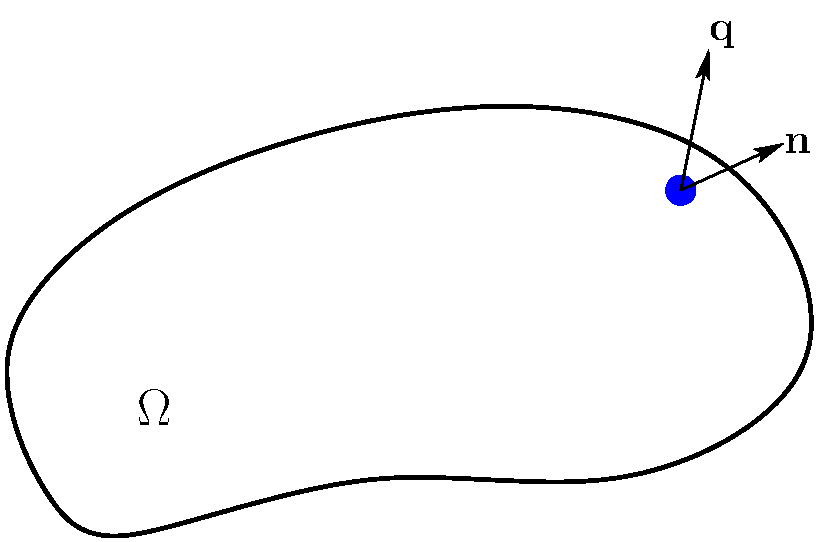
\includegraphics[scale=0.5]{HeatFlux}
  \end{center}
  \caption{
    The domain $\Omega$ and a surface element on the boundary
    $\partial\Omega$. The outward unit normal vector ${\bm n}$ is indicated,
    together with the heat flux ${\bm q}$.
  }
  \label{fig:HeatFlux}
\end{figure}

In the case of constant thermal diffusivity $\kappa$, the governing equation
reduces to the Poisson equation
\begin{align}
  \label{steady-heat}
  - \kappa\nabla^2 u = f.
\end{align}

\section {Unsteady Heat Transfer Problems}

Assuming no fluid flow, energy conservation in the unsteady case is described by
the the unsteady (parabolic) heat equation
\begin{align}
  \label{heat-eq}
  \frac{\partial u}{\partial t}
  = \kappa \nabla^2 u + f \qquad \text{in}\,\Omega.
\end{align}

If we discretize this equation in time using the Euler Backward method, we
obtain
\begin{align}
  \frac{u^{n+1}- u^n}{\Delta t}
  = \kappa\nabla^2 u^{n+1} + f^{n+1},
\end{align}
where superscript $n$ refers to a quantity at time $t^n,\, n=0,1,2,\ldots$. This
can also be expressed as
\begin{align}
  \label{helm-eq}
  \left[- \kappa\nabla^2 +\frac{1}{\Delta t} \right] u^{n+1} =
  \frac{u^n}{\Delta t} + f^{n+1}.
\end{align}
Hence, a typical evolution problem discretized in time using implicit finite
differences will necessitate the solution of a Helmholtz type equation at each
time step. Note that the Helmholtz operator (the operator inside the
parentheses) corresponds to the Laplace operator plus a multiple of the identity
operator.

\section{Eigenvalue problems}

Eigenvalue calculations also form an important application area in science and
engineering. A typical example is the computation of the first eigenmodes or
eigenvibrations in a structure, e.g. a building, a bridge or a turbine. In
order to avoid resonance phenomena in the structure, one can precompute the most
important eigenmodes numerically, and design the structure such that resonance
is avoided for a typical external load or excitation.

To illustrate a typical analysis, consider the following simple model problem:
\begin{align*}
  -\nabla^2 u = \lambda u
\end{align*}
with proper boundary conditions, e.g. the solution specified along the domain
boundary. A numerical model is then constructed for this eigenvalue problem.
This discretization will typically result in a large set of algebraic equations.
The smallest eigenvalues/eigenmodes will give information of \emph{physical
significance}; for our specific model problem, they will approximate the
eigenmodes for a diffusive system and the time constants associated with the
decay of these.

\section{Outputs from partial differential equations}

In many engineering applications, the primary interest may not be the details of
the solution $u$ everywhere in the domain $\Omega$, but rather some very
specific output, e.g. the average temperature over part of the domain boundary,
the drag on an underwater cable due to currents in the sea, or an eigenvalue
(e.g. the lowest eigenfrequency). In these cases, the ultimate interest may
just be a single number. However, in order to compute this output of interest, a
numerical approximation $u_h$ to $u$ needs to be computed on the entire
computational domain $\Omega$, perhaps involving thousands or millions of
unknowns.

\section{Other important issues}

There are many topics that are important in order to successfully obtain
accurate numerical solutions for realistic physical problems.

\subsection{Grid generation}

In this course, we will primarily consider problems in one and two space
dimensions. In one space dimension, the grid generation is trivial. However, for
realistic two and three-dimensional domains, the grid generation itself may pose
a major challenge. In the past, there has been much effort put into the
construction of automatic mesh generators, however, this is still an ongoing
research topic. It turns out that it is easier to decompose a general
computational domain into triangles and tetrahedral elements than it is to
decompose it into quadrilateral or hexahedral elements. This is the main reason
why the use of triangular and tetrahedral (finite) elements tends to be fairly
popular for representing general geometries; e.g. see \autoref{fig:dd_grid}.

\begin{figure}[htbp]
  \begin{center}
    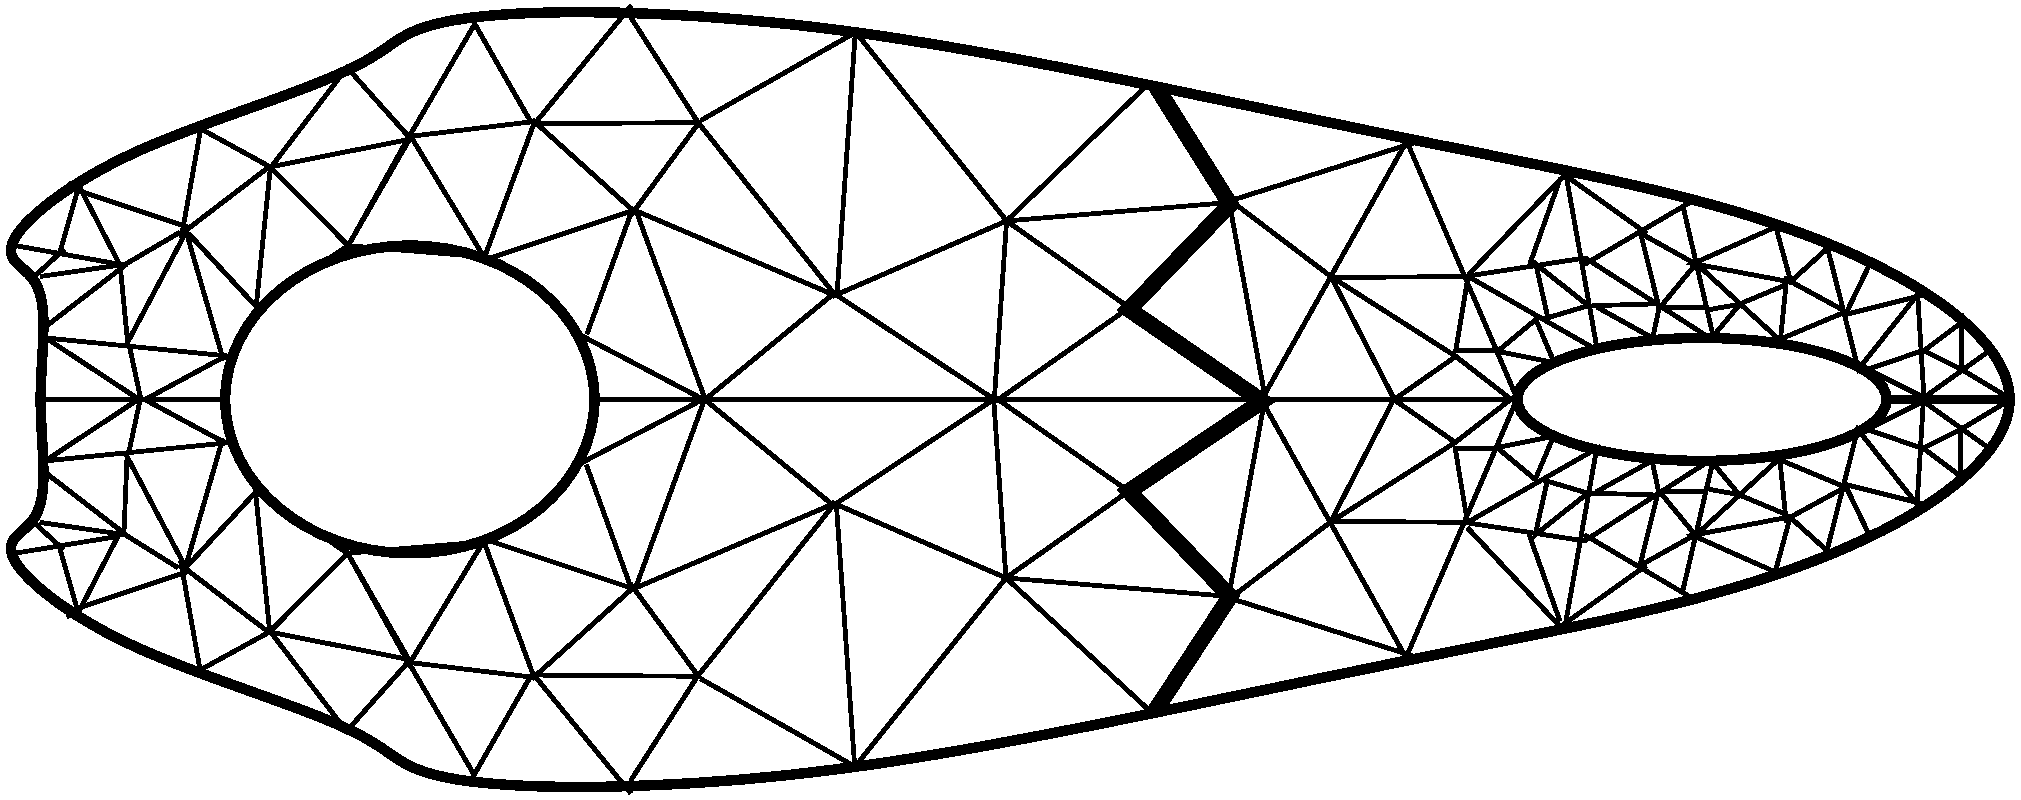
\includegraphics[scale=0.25]{dd_grid}
  \end{center}
  \caption{
    A triangulation of a two-dimensional domains and a partitioning of this
    domain into two subdomains (the bold line represents the subdomain
    interface).
  }
  \label{fig:dd_grid}
\end{figure}

We will not focus on these issues in this course, and stick to simple,
rectangular domains with cartesian meshes.

\subsection{Domain decomposition and parallel computing}

A second important issue related to grid generation is \emph{domain
decomposition}. This is the decompostion of the computational grid into
subdomains, where each subdomain again represents many degrees-of-freedom; see
\autoref{fig:dd_grid}.

Domain decomposition may be important for several reasons. If one is interested
in using a parallel computer with a distributed memory, the global problem
(including the grid) needs to be distributed among the processors. In this
context, each individual subdomain may be associated with a single processor.
However, even on a single process computer, domain decomposition may prove very
useful in the construction of preconditioners for iterative solution methods,
i.e. methods that will speed up the convergence rate when solving the system of
algebraic equations.

Creating a good decomposition from a given grid is not always a trivial task for
general meshes. This is also a field where much progress has been made over the
past few years.

We will come back to this in the course, both in the context of solving the
discretized equation using parallel computers as well as in the context of
preconditioner construction.

\subsection{Adaptivity}

For complex problems, the initial grid is typically generated such that areas
where one expects the solution to exhibit large gradients are well resolved
(i.e. a higher density of elements or degrees-of-freedom is used in those
areas). This approach is very heuristic, and the quality of the underlying mesh
depends strongly on how well one is able to predict the solution structure.

An improved strategy is to use the initial (perhaps coarse) mesh to obtain a
temporary solution which is subsequently used for the purpose of refining the
mesh where the error is expected (or estimated) to be large. This is called
\emph{a posteriori} error estimation and \emph{adaptive} grid refinement (or
perhaps unrefinement). It is an area of considerable research effort since it
promises better error control and reduced computational cost for a fixed error
target. However, adaptive grid refinement is not a trivial task to analyze or to
implement, in particular, for unsteady problems where the solution structure may
change as a function of time.

We will not focus on adaptivity in this course.

\subsection{Visualization}

Once a numerical solution has been computed, the computational results need to
be interpreted. For a multi-dimensional problem, one typically ends up with a
large amount of data. Visualization of these data is often essential in order to
extract useful information from the simulation. Even though the final answer we
are looking for may just be a single number (e.g. the drag), we often want to
understand some of the main features in the solution. With huge amount of data,
visualization (including feature extraction) are invaluable tools. In the
context of parallel computing, visualization is particularly important due to
the very high volume of raw data.

We will consider how to handle the output in this course, but will not focus on
visualization tools. Matlab and Octave will suffice for our needs.

\subsection{Software development}

The effort needed to design and implement a software package for large-scale
simulation of physical systems is typically significant. The associated cost is
therefore also very high. Hence, it is very important to consider good ways to
break down the global problem into smaller modules which can interact in a
flexible and efficient manner.

The use of \emph{object-oriented design} has become popular in recent years. One
of the key issues when designing and implementing a large software package is to
be able to identify commonalities between the various computational tasks, and
to properly encapsulate these so that they may be made into more generic modules
which can be reused for different purposes. An example of this is the solution
of the Poisson equation, which may be used for multiple purposes in the same
simulation package. Another key issue is the concept of data abstraction where
one tries to implement higher-level functionality without necessarily having to
worry about all the details in the lower-level tasks.

\section{Final comments}

It is common to consider the numerical solution of partial differential
equations in the following conceptual model:
\begin{enumerate}
\item we know the computational domain $\Omega$ and the various parameters and
  input data (e.g. the thermal diffusivity $\kappa$ and the volumetric heat
  source $f$);
\item we compute a discrete approximation over the entire domain;
\item we compute the actual output of interest and otherwise interpret and
  visualize the results.
\end{enumerate}

The above approach is often referred to as a \emph{forward problem}, and it may
be sufficient for many problems. However, for certain applications, this mode of
analysis and computation will not suffice. We may not always know the precise
shape of the computational domain, e.g. an airplane wing. In fact, finding the
shape which minimizes the drag may be part of the objective with the simulation.
In such a case, many forward problems are solved, each one hopefully getting
closer to an optimal solution. This type of application represents an example of
an optimization problem. In this context, we note that computing the solution of
a partial differential equation may only give a single data point in a larger
optimization algorithm.

Another area where numerous forward problems may be required is for applications
where the input parameters (e.g. the thermal diffusivity $\kappa$) are not
known, but in fact the quantity of main interest. For such applications, one
will typically have available a certain number of \emph{measurements}
corresponding to multiple \emph{outputs} from the governing equation. The
objective is then to find a distribution of the thermal diffusivity inside the
computational domain such that the difference between the simulated outputs and
the real, physical outputs (or measurements) is minimized. This type of
application represents an example of an \emph{inverse problem}, and is of
significant importance in areas such as medical imaging, estimation of rock
properties etc.
